\documentclass[conference]{IEEEtran}
\IEEEoverridecommandlockouts

\usepackage{cite}
\usepackage{amsmath,amssymb}
\usepackage{graphicx}
\usepackage{booktabs}
\usepackage{multirow}
\usepackage{xcolor}
\usepackage{url}
\usepackage{tikz}
\usetikzlibrary{arrows.meta,positioning,fit}
\graphicspath{{../figures/}}

\begin{document}

\title{Svelto-DNA: Interactive Splice-Disruption Analysis on a Frozen Genomic Foundation Model with Speculative In-Silico Mutagenesis}

% Affiliations and e-mail addresses: fill in before submission.
\author{\IEEEauthorblockN{Derrick Rajkumar}
\and
\IEEEauthorblockN{Yuvaraj R.}}

\maketitle

\begin{abstract}
Splice-altering variants are a frequent and under-diagnosed cause of genetic disease, and deep sequence models can score them, but exhaustive in-silico mutagenesis (ISM) of a region requires one forward pass per candidate substitution, which makes interactive exploration slow. We present Svelto-DNA, an open system that pairs a frozen HyenaDNA backbone with a small trained splice-site head, a validated vectorized splice-disruption ($\Delta$) calculator, a WebSocket scoring service, and a browser-based explorer. Because HyenaDNA is causal, the head reads forward and reverse-complement features so that every position sees both flanks. On held-out chromosomes (62.7\,M positions, 112{,}019 annotated sites) the model reaches donor/acceptor PR-AUC 0.630/0.552 and ROC-AUC 0.9989/0.9984. Fed SpliceAI's own probability tracks, our $\Delta$ calculator reproduces published SpliceAI scores for eight ClinVar pathogenic variants within their 3-decimal rounding. To accelerate ISM we evaluate a speculative draft-and-verify scheme: one reference pass drafts which candidates could matter and only the top-$K$ are verified exactly in batched passes. On a laptop GPU, exact batched verification gives only $1.2\times$; larger speedups come solely from verifying fewer candidates and cost recall ($2.4\times$ at 0.83 recall of high-impact variants, $9.1\times$ at 0.31). We report these trade-offs, and two negative results, so that speculative claims for genomic models can be judged against recall rather than speed alone.
\end{abstract}

\begin{IEEEkeywords}
RNA splicing, variant effect prediction, genomic foundation models, HyenaDNA, in-silico mutagenesis, speculative decoding, ClinVar
\end{IEEEkeywords}

\section{Introduction}
Pre-mRNA splicing is directed by short sequence signals: a GT dinucleotide at the 5$'$ (donor) end of an intron, an AG at its 3$'$ (acceptor) end, and surrounding consensus and regulatory sequence. Single-nucleotide variants that destroy these signals or create cryptic ones can skip exons, shift splice boundaries and disrupt reading frames, and such variants are a recurring cause of inherited disease~\cite{scotti2016missplicing}. A classic example is \textit{MAPT} exon~10, where mutations near the exon~10 donor alter tau isoform ratios and cause frontotemporal dementia (FTDP-17)~\cite{hutton1998ftdp17}.

Deep models now predict splicing from sequence with high accuracy: SpliceAI~\cite{jaganathan2019spliceai} and Pangolin~\cite{zeng2022pangolin} score the effect of a variant as the change ($\Delta$) in predicted site probabilities within a local window. Genomic foundation models such as HyenaDNA~\cite{nguyen2023hyenadna} and the Nucleotide Transformer~\cite{dallatorre2025nt} offer general-purpose sequence representations that can be adapted to such tasks. Exploring a region with these models remains slow, however: in-silico saturation mutagenesis (ISM)~\cite{alipanahi2015deepbind} needs one forward pass per candidate substitution, i.e.\ $3n$ passes for $n$ positions.

In language models, speculative decoding~\cite{leviathan2023speculative,chen2023speculative} and multi-head drafting~\cite{cai2024medusa} cut latency by drafting cheaply and verifying in parallel. We ask whether the same idea helps variant scanning, and build a complete system to measure it. Our contributions are:
\begin{itemize}
  \item an open pipeline from GENCODE, GRCh38 and ClinVar to chromosome-disjoint splice-site datasets, with fixes to two silent data errors we found along the way (Section~\ref{sec:data});
  \item a splice-site head on a \emph{frozen} HyenaDNA backbone that combines forward and reverse-complement features to compensate for the backbone's causality (Section~\ref{sec:model});
  \item a vectorized $\Delta$ calculator validated against published SpliceAI scores (Section~\ref{sec:delta});
  \item speculative ISM with exact batched verification, measured honestly against both sequential and batched exhaustive baselines, with recall as a first-class metric (Sections~\ref{sec:spec} and~\ref{sec:results});
  \item an interactive WebSocket service and browser explorer for clinicians (Section~\ref{sec:system}).
\end{itemize}

\section{Related Work}
\textbf{Splice prediction.} MaxEntScan~\cite{yeo2004maxent} scores short splice motifs with maximum-entropy models. SpliceAI~\cite{jaganathan2019spliceai} trained a 10\,kb-context residual CNN end to end and introduced the $\Delta$ score used here; Pangolin~\cite{zeng2022pangolin} extended this to tissue-specific usage. The Broad SpliceAI-lookup service~\cite{spliceailookup} publishes precomputed scores that we use as ground truth.

\textbf{Genomic foundation models.} HyenaDNA~\cite{nguyen2023hyenadna} replaces attention with Hyena long convolutions~\cite{poli2023hyena}, giving single-nucleotide tokens and long context. The Nucleotide Transformer~\cite{dallatorre2025nt} uses attention over 6-mer tokens. Enformer~\cite{avsec2021enformer} combines convolutions and attention for expression prediction.

\textbf{Speculative inference.} Speculative decoding~\cite{leviathan2023speculative,chen2023speculative} drafts tokens with a cheap model and verifies them with the target model; Medusa~\cite{cai2024medusa} drafts with extra heads and verifies a candidate tree with tree attention. HyenaDNA has no attention, so tree-masked verification does not apply; we instead speculate at the level of whole variants.

\textbf{Attribution.} Gradient-based saliency~\cite{simonyan2013saliency} and gradient $\times$ input~\cite{shrikumar2017deeplift} explain which inputs drive a prediction; we use the latter to show which bases support a predicted splice site.

\section{Data}\label{sec:data}
We use GENCODE v46 basic annotation~\cite{frankish2023gencode}, keeping one canonical protein-coding transcript per gene (\texttt{Ensembl\_canonical}): 19{,}120 transcripts on chr1--22 with 366{,}000 splice sites. Sequence comes from the Ensembl GRCh38 primary assembly~\cite{harrison2024ensembl}. Training examples are transcript-oriented windows: a 1\,kb labelled block with 1\,kb of flank on each side. Minus-strand genes are reverse-complemented, and each site is labelled on the first base of its dinucleotide (G of GT, A of AG). All blocks that contain a site are kept, plus one site-free block per transcript, so positives are enriched relative to the genome. Splits are by chromosome with zero chromosome and gene overlap: train chr11--22 (86{,}811 windows), validation chr2,4,6,8,10 (51{,}657) and test chr1,3,5,7,9 (62{,}739).

From the ClinVar GRCh38 release~\cite{landrum2018clinvar} we keep SNVs within $\pm$50\,bp of an annotated site (2{,}118{,}576 variants) and label them by clinical significance. Two silent errors were found and fixed. First, real ClinVar records carry no junction distance; a parser that defaulted the distance to zero let every SNV pass the $\pm$50\,bp filter, so distances are now computed from exon coordinates. Second, ClinVar's 2024 wording ``Conflicting classifications of pathogenicity'' contains the word ``pathogenic''; substring matching labelled 86{,}949 conflicting variants as pathogenic. After the fix, 119{,}787 variants are pathogenic or likely pathogenic, 732{,}647 benign or likely benign, and 1{,}266{,}142 (uncertain or conflicting) are held out.

\section{Model}\label{sec:model}
The backbone is HyenaDNA-small-32k (3.28\,M parameters, $D=256$, 4 layers), loaded with its own single-nucleotide vocabulary and kept frozen. Weights stay in fp32 and inference uses fp16 autocast, which matches fp32 outputs with cosine similarity 0.99998 on a 10\,kb window.

HyenaDNA is causal: the state at position $t$ depends only on bases $\le t$, but a donor depends on the intron sequence downstream of it. We therefore run the backbone on both strands and align the reverse-complement pass back to forward coordinates:
\begin{equation}
h_t = \big[\, H(x)_t \;;\; H(\mathrm{rc}(x))_{L-1-t} \,\big] \in \mathbb{R}^{2D}.
\end{equation}
After a single-base edit 50\,bp downstream of position $t$, the forward half of $h_t$ changes only by FFT round-off ($\sim3\times10^{-3}$), while the reverse-complement half changes 80--300$\times$ more, confirming that the second pass supplies the missing downstream context.

A two-hidden-layer MLP (LayerNorm, GELU, width 256) maps $h_t$ to $p_t=\mathrm{softmax}(f(h_t))$ over \{neither, donor, acceptor\}. Only the head is trained, with class-weighted cross-entropy (weight 20 on the two site classes) over each labelled block, AdamW (learning rate $10^{-3}$) and a one-cycle schedule, for 4{,}000 steps of 16 windows. Training takes 14 minutes on an NVIDIA RTX~5060 Laptop GPU, and the checkpoint with the best mean validation PR-AUC (0.574) is kept.

\begin{figure}[t]
\centering
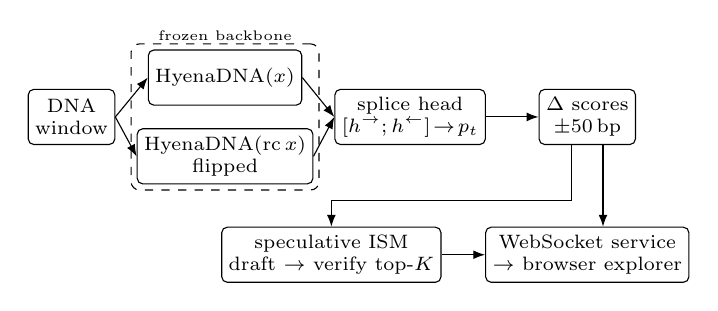
\begin{tikzpicture}[font=\scriptsize,
  box/.style={draw, rounded corners=2pt, align=center, minimum height=7mm, inner sep=2.5pt},
  arr/.style={-{Latex[length=1.5mm]}}]
\node[box] (x) at (0,0) {DNA\\window};
\node[box, minimum width=19mm] (f) at (1.95,0.5) {HyenaDNA$(x)$};
\node[box, minimum width=19mm] (r) at (1.95,-0.5) {HyenaDNA$(\mathrm{rc}\,x)$\\flipped};
\node[box] (h) at (4.3,0) {splice head\\$[h^{\rightarrow};h^{\leftarrow}]\!\to\!p_t$};
\node[box] (d) at (6.55,0) {$\Delta$ scores\\$\pm$50\,bp};
\node[box] (s) at (3.3,-1.75) {speculative ISM\\draft $\to$ verify top-$K$};
\node[box] (ws) at (6.55,-1.75) {WebSocket service\\$\to$ browser explorer};
\node[draw, dashed, rounded corners=3pt, inner sep=2pt, fit=(f)(r), label={[font=\tiny, inner sep=1pt]above:frozen backbone}] {};
\draw[arr] (x.east) -- (f.west); \draw[arr] (x.east) -- (r.west);
\draw[arr] (f.east) -- (h.west); \draw[arr] (r.east) -- (h.west);
\draw[arr] (h) -- (d);
\draw[arr] ([xshift=-2mm]d.south) -- ++(0,-0.7) -| (s.north);
\draw[arr] (d.south -| ws.north) ++(2mm,0) -- ([xshift=2mm]ws.north);
\draw[arr] (s) -- (ws);
\end{tikzpicture}
\caption{Svelto-DNA overview. The frozen backbone runs on both strands; a trained head predicts per-base site probabilities, from which $\Delta$ scores, speculative scans and the interactive service are built.}
\label{fig:overview}
\end{figure}

\section{Variant Effect and Its Validation}\label{sec:delta}
For a variant at $v$ with reference and mutant tracks $p^{\mathrm{ref}},p^{\mathrm{mut}}$ and window $W=50$, we follow SpliceAI:
\begin{align}
\Delta_{\mathrm{DG}} &= \max_{|j-v|\le W} \big(p^{\mathrm{mut}}_{j,\mathrm{d}} - p^{\mathrm{ref}}_{j,\mathrm{d}}\big),\\
\Delta_{\mathrm{DL}} &= \max_{|j-v|\le W} \big(p^{\mathrm{ref}}_{j,\mathrm{d}} - p^{\mathrm{mut}}_{j,\mathrm{d}}\big),
\end{align}
with $\Delta_{\mathrm{AG}},\Delta_{\mathrm{AL}}$ defined analogously for acceptors and $\Delta=\max(\Delta_{\mathrm{DG}},\Delta_{\mathrm{DL}},\Delta_{\mathrm{AG}},\Delta_{\mathrm{AL}})$. All four components are computed at once with a 1D max-pool over the stacked differences.

To validate the calculator independently of our model, we ran the official SpliceAI five-model ensemble on reference and mutant windows for eight ClinVar \emph{pathogenic} canonical-site SNVs (four per strand, donors and acceptors) and fed its full $\pm$50\,bp tracks to our implementation. All 32 component scores match the scores published by SpliceAI-lookup~\cite{spliceailookup} with a maximum absolute difference of 0.000476, inside the $\pm$0.0005 of their 3-decimal rounding, and every peak position matches exactly. The calculator takes 0.21\,ms for a 10\,kb window on the GPU and 0.55\,ms on the CPU.

\section{Speculative In-Silico Mutagenesis}\label{sec:spec}
For a window of $n$ positions the candidate set $C$ contains every alternative base, $N=|C|=3n$. \emph{Vanilla} ISM scores each candidate with its own forward pass. \emph{Speculative} ISM (i) runs one reference pass; (ii) ranks candidates with a draft score computed without the model,
\begin{equation}
d(c)=\max\big(s_{\mathrm{on}}(c),\; s_{\mathrm{near}}(c),\; 0.5\cdot\mathbb{1}[c\ \text{creates GT/AG}]\big),
\end{equation}
where $s_{\mathrm{on}}$ is the reference site probability on the dinucleotide hit by $c$ and $s_{\mathrm{near}}$ the strongest nearby site probability with decay $e^{-|j-v|/4}$; and (iii) verifies the top-$K$ candidates exactly in batched passes. Unverified candidates are reported as unknown, never as zero.

A variant is high-impact if $|\Delta|\ge\tau$ with $\tau=0.2$. We report the acceptance rate $\alpha$ (fraction of verified candidates that are high-impact), the recall of high-impact variants relative to exhaustive ISM, wall-clock speedup against both sequential and batched exhaustive ISM, and the fraction of forward passes saved, $1-(1+K)/(1+N)$. Batched verification equals sequential verification within $6\times10^{-8}$ in fp32 and within $4.1\times10^{-3}$ under fp16 autocast.

\section{Interactive System}\label{sec:system}
A FastAPI WebSocket service exposes \texttt{mutate}, \texttt{score}, \texttt{reset} and \texttt{scan} actions per session. Edits apply to the session state immediately; scoring runs on a single GPU worker, and a queued request is skipped if a newer edit for the same session has arrived, so stale work is avoided rather than hidden. Each response carries per-base reference and mutant probabilities, the four $\Delta$ tracks and measured latency. A Next.js explorer renders a virtualized 10\,kb sequence ribbon, reference and mutant tracks, and a continuous zoom from a whole-brain view to the base pair; it sustains 57--60 frames per second on the same laptop GPU. With the real backbone and head, a 1\,kb edit takes a median of 12.5\,ms round trip (p95 13.9\,ms).

\section{Results}\label{sec:results}

\subsection{Splice-site prediction}
Table~\ref{tab:pred} reports held-out test performance (chr1,3,5,7,9; 62.7\,M positions, 56{,}008 donors, 56{,}011 acceptors; non-site to site ratio 559:1). The untrained head scores PR-AUC 0.0007, i.e.\ chance. For context, SpliceAI-10k reports top-1 accuracy around 0.95 with 10\,kb of context and end-to-end training~\cite{jaganathan2019spliceai}; our model is a frozen 3.3\,M-parameter backbone with 1\,kb flanks and a small head, and we present it as a baseline rather than a competitor.

\begin{table}[t]
\centering
\caption{Splice-site prediction on held-out chromosomes}
\label{tab:pred}
\begin{tabular}{lcc}
\toprule
 & Donor & Acceptor \\
\midrule
ROC-AUC & 0.9989 & 0.9984 \\
PR-AUC & 0.6295 & 0.5520 \\
Top-1 accuracy & 0.604 & 0.542 \\
Top-2$k$ accuracy & 0.811 & 0.738 \\
\bottomrule
\end{tabular}
\end{table}

\subsection{Speculative ISM}
Table~\ref{tab:spec} summarizes 40 held-out windows, each a 64\,bp scan region (192 candidates) inside 2.2\,kb of sequence. Exact batched verification is only $1.2\times$ faster than sequential ISM: profiling shows that HyenaDNA-small saturates this GPU at a batch of 2--4 sequences ($\approx$2.3\,ms per sequence per pass, versus 3.07\,ms at batch 1 and 3.24\,ms at batch 64). Every larger speedup therefore comes from verifying fewer candidates. At $K=96$ the scan is $2.38\times$ faster than sequential ISM and finds 83\% of the high-impact variants on average (57\% in the worst window); at $K=24$ it is $9.1\times$ faster but finds only 31\%.

\begin{table}[t]
\centering
\caption{Speculative ISM on 40 held-out windows (64\,bp scan region in 2{,}164\,bp of sequence, 192 candidates, $|\Delta|\ge0.2$). Speedup is relative to sequential ISM.}
\label{tab:spec}
\setlength{\tabcolsep}{4pt}
\begin{tabular}{lrrrr}
\toprule
Method & ms & Speedup & Recall & $\alpha$ \\
\midrule
Sequential & 1346 & 1.00$\times$ & 1.00 & -- \\
Batched exhaustive & 1126 & 1.20$\times$ & 1.00 & -- \\
Speculative $K{=}96$ & 567 & 2.38$\times$ & 0.83 & 0.26 \\
Speculative $K{=}48$ & 287 & 4.68$\times$ & 0.51 & 0.30 \\
Speculative $K{=}24$ & 148 & 9.10$\times$ & 0.31 & 0.38 \\
\bottomrule
\end{tabular}
\end{table}

Fig.~\ref{fig:ablation} extends this to three sequence lengths (664, 1{,}164 and 2{,}164\,bp, all real sequence; 16 windows each). Recall is stable across lengths, with mean values of 0.28, 0.39, 0.60 and 0.87 at $K=12, 24, 48, 96$. The ablation's timings were recorded on battery power in a power-saving profile, which slows the overhead-bound batch-1 path; its absolute speedups are therefore larger than in Table~\ref{tab:spec} and should be read relative to one another.

\begin{figure}[t]
\centering
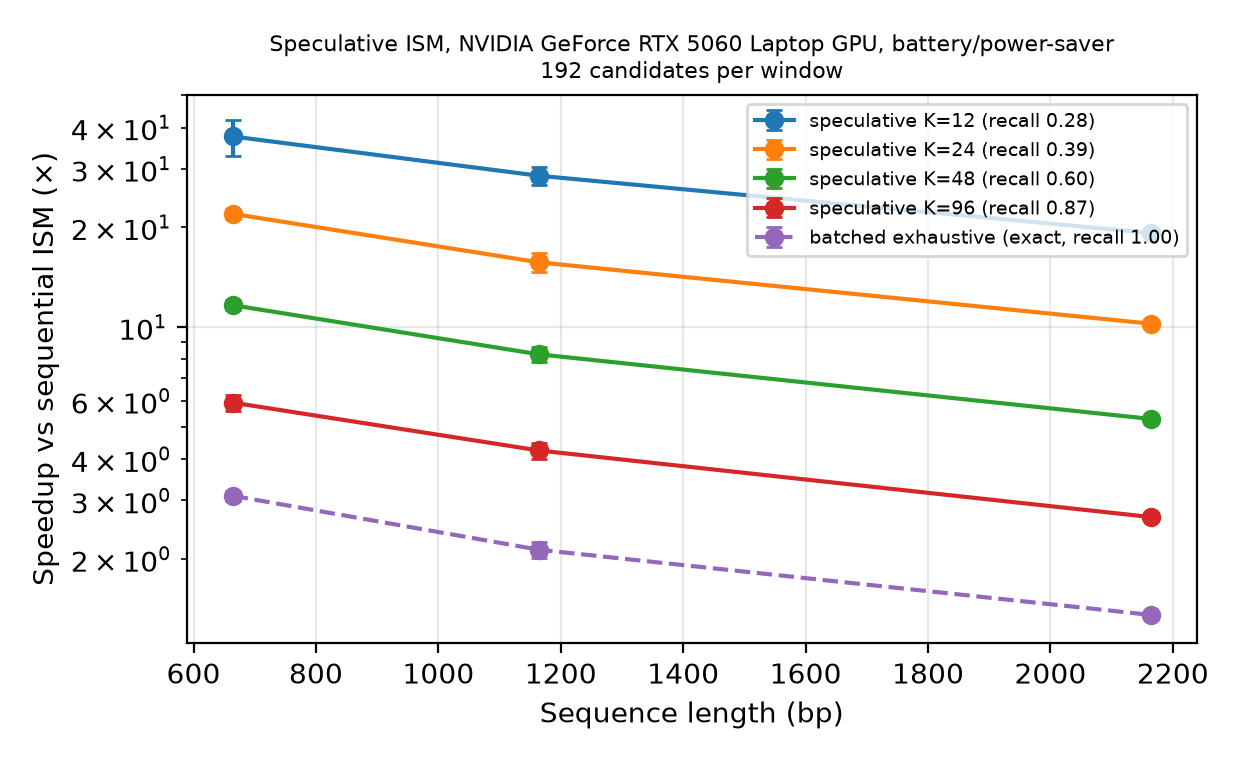
\includegraphics[width=0.92\columnwidth]{speedup_vs_length.png}\\[1mm]
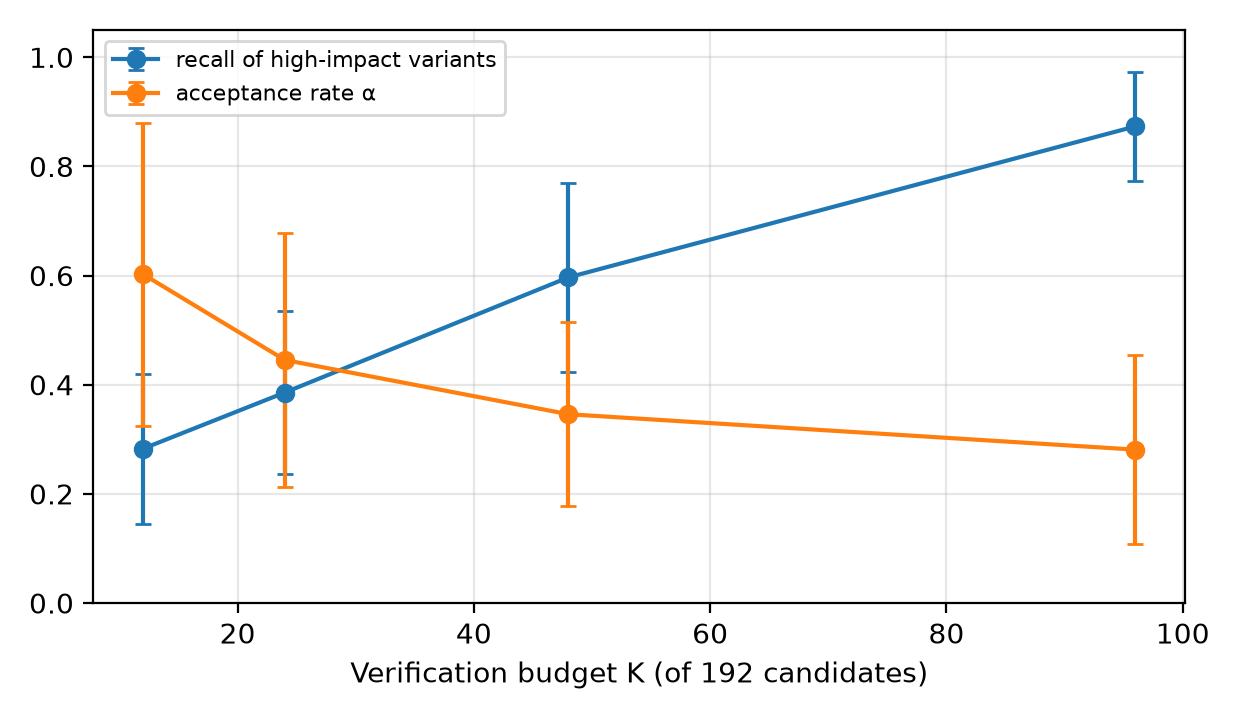
\includegraphics[width=0.92\columnwidth]{recall_alpha_vs_k.png}
\caption{Top: speedup over sequential ISM against sequence length, mean $\pm$ s.d.\ over 16 windows; the legend gives each budget's recall. Bottom: recall and acceptance rate against the verification budget $K$. Timings were recorded on battery in a power-saving profile.}
\label{fig:ablation}
\end{figure}

\subsection{Case study}
Fig.~\ref{fig:case} shows ClinVar variant 635252 in \textit{ABAT} (chr16:8{,}746{,}099 G$>$A), which hits the first base of a donor GT. Our model predicts donor loss $\Delta_{\mathrm{DL}}=0.937$ (SpliceAI: 0.996). For ClinVar 1983599 in \textit{ABCG8} (chr2:43{,}852{,}353 G$>$C), the G of an acceptor AG, it predicts acceptor loss $\Delta_{\mathrm{AL}}=0.840$ (SpliceAI: 0.936). Peak positions differ from SpliceAI's by 1--2\,bp because the two models place site labels on different bases (we label the first base of the dinucleotide, SpliceAI the exon-side boundary). Saliency concentrates on the dinucleotide and its immediate consensus positions.

\begin{figure}[t]
\centering
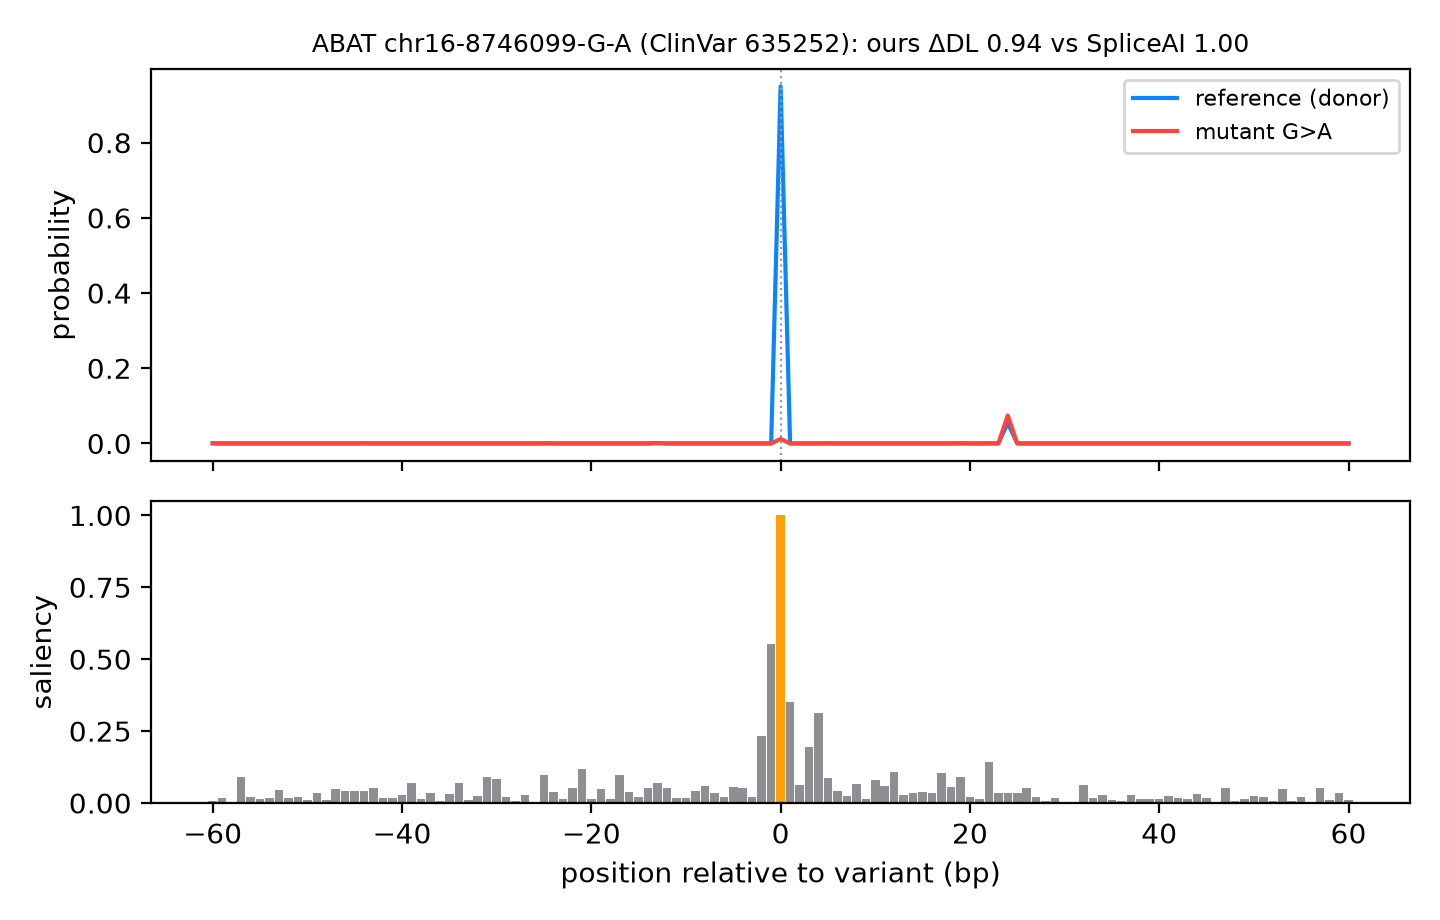
\includegraphics[width=0.92\columnwidth]{case_ABAT.png}
\caption{\textit{ABAT} chr16:8{,}746{,}099 G$>$A (ClinVar 635252). Top: donor probability for reference and mutant. Bottom: gradient$\times$input saliency of the reference donor site; the variant position is highlighted.}
\label{fig:case}
\end{figure}

\section{Discussion and Limitations}
\textbf{Speed versus recall.} Speculative verification is exact for the candidates it verifies, but in variant scanning the cost of a missed high-impact variant is clinical, not cosmetic. On our hardware, the honest summary is $1.2\times$ with no missed variants, or roughly $2.4\times$ while missing about one in six. Unlike token-level speculative decoding, where rejected drafts are regenerated and outputs stay identical, an unverified variant here is simply unknown.

\textbf{Negative results.} A first-order gradient draft, scoring each substitution by $|\nabla_e S\cdot(e_{\mathrm{alt}}-e_{\mathrm{ref}})|$ for the splice mass $S$ near the window, did not beat the heuristic draft (recall 0.65 versus 0.83 at $K=96$ on 16 windows). Padding windows with N to emulate longer contexts pushed the model out of distribution: it predicted no sites, so recall was undefined, and we report only real-sequence lengths.

\textbf{Limitations.} Paralogs are not removed from the test set, so some test genes may resemble training genes. The model sees only 1\,kb flanks, well below SpliceAI's 10\,kb. All timings come from one laptop GPU, and wall-clock results depend on its power state. The browser demo shows a synthetic region by default, although the service can serve real GRCh38 windows.

\section{Conclusion}
Svelto-DNA turns a frozen genomic foundation model into an interactive splice-disruption tool with validated $\Delta$ scores and sub-15\,ms edits. Speculative in-silico mutagenesis offers a tunable trade between speed and recall rather than a free speedup, and we recommend that speculative methods for genomic models always report recall against exhaustive scanning. Next steps are longer context, a learned variant-effect drafter trained on ISM labels, and evaluation on server-class GPUs where batching may amortize better.

\section*{Code and Data Availability}
Code, scripts and measured results are in the Svelto-DNA repository. Every number in this paper is produced by a committed script from public GENCODE, Ensembl and ClinVar data.

\bibliographystyle{IEEEtran}
\bibliography{refs}

\end{document}
